\begin{figure}[!h]
    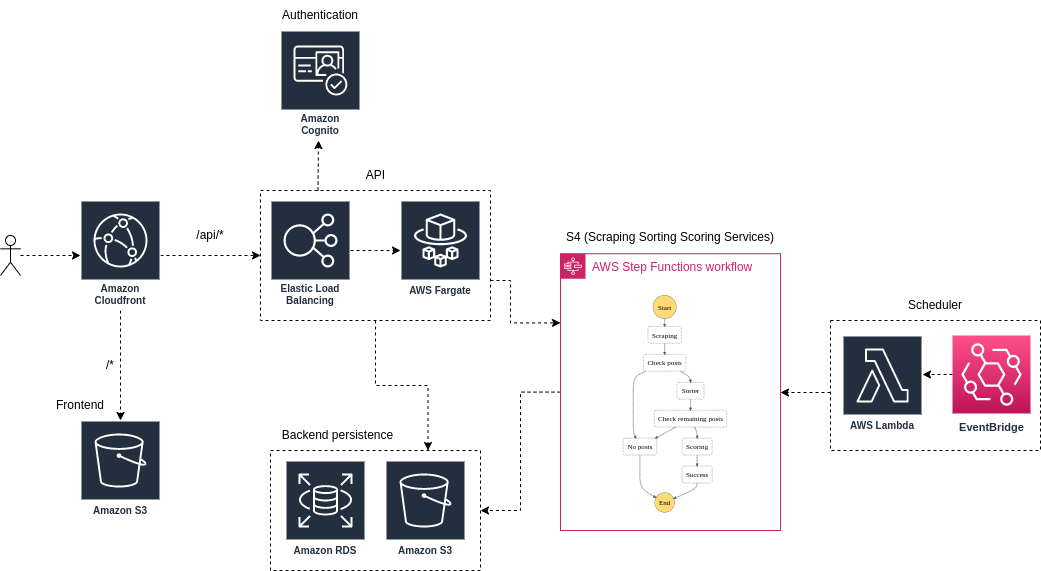
\includegraphics[width=16cm]{sezioni/images/overview.png}
    \centering
    \caption{Visione d'insieme del sistema}
\end{figure}

\subsection{Descrizione generale}
Il Backend della piattaforma sfrutta un'architettura a microservizi, i quali comunicano fra di loro secondo regole e meccanismi appropriati.
Le varie parti sono fra di loro indipendenti e i dati da esse prodotti persistono in RDS o bucket S3, a seconda della lora natura.
Il lavoro di analisi e progettazione ha permesso di individuare i seguenti servizi:
\begin{itemize}
    \item \textbf{API Service}: ha il compito di far interfacciare il Frontend con il resto del sistema, in particolare fornisce
    delle API RESTful che consentono l'ottenimento dei dati dal database e in generale di gestire tutte le funzionalità rese disponibili all'utente;
    \item \textbf{Signup Service}: risponde agli eventi \textit{pre signup} di Cognito e permette di aggiungere automaticamente utenti al database della piattaforma, dopo la loro registrazione;
    \item \textbf{S4} (\textbf{S}craping \textbf{S}orting \textbf{S}coring \textbf{S}ervices):
        \begin{itemize}
            \item \textbf{Scraping Service}: sfruttando apposite tecniche e librerie, effettua operazioni di scraping da Instagram al fine di ottenere dati che
            saranno successivamente processati dagli altri servizi;
            \item \textbf{Sorting Service}: effettua un preprocessing sui dati ottenuti dallo scraping, scartando eventuali dati non conformi e che comporterebbero
            uno spreco di risorse nelle fasi successive di analisi;
            \item \textbf{Scoring Service}: esegue analisi approfondite su dati testuali e multimediali, producendo una valutazione numerica; 
        \end{itemize}
    \item \textbf{Scheduler Service}: programma l'esecuzione di \textbf{S4} secondo un intervallo di tempo predefinito.
\end{itemize}

\subsection{Servizi S4}
I servizi di scraping, sorting e scoring formano un raggruppamento logico chiamato \textbf{S4} (\textbf{S}craping \textbf{S}orting \textbf{S}coring \textbf{S}ervices).
Essi vengono eseguiti in funzioni Lambda, le quali sono orchestrate attraverso \textit{AWS Step Functions}.
\begin{figure}[H]
    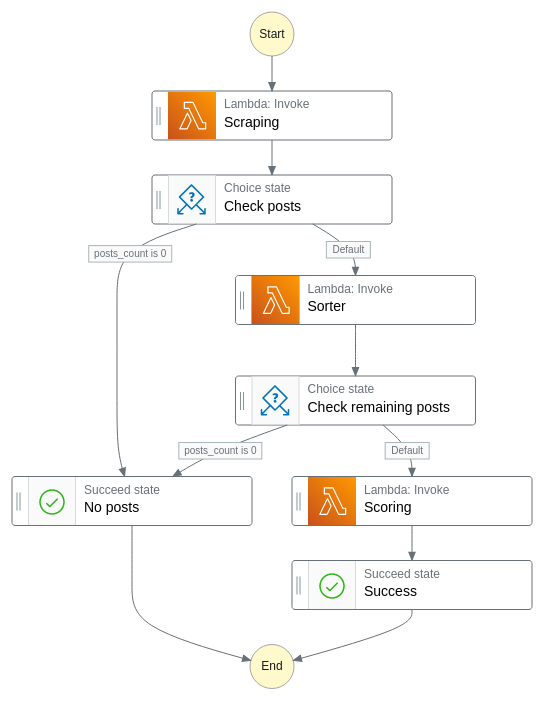
\includegraphics[width=8cm]{sezioni/images/stepfunctions_graph.png}
    \centering
    \caption{Visualizzazione macchina a stati}
\end{figure}
L'orchestratore permette di definire il flusso di esecuzione come una macchina a stati, dove l'output di uno stato
diventa l'input di quello successivo.\\
Uno stato può anche controllare il flusso dell'esecuzione, per esempio se dopo
l'operazione di sorting non restano post da analizzare e quindi da passare in input al servizio di scoring, si arriva
subito ad uno stato terminale che quindi termina l'esecuzione senza sprecare risorse.
